%!TEX root =../mapp-challenge-18-game-book.tex
% ^ leave for LaTeXTools build functionality

\phChapterWorksheet{The Kantor Region}{Opening Puzzle}



\begin{center}
  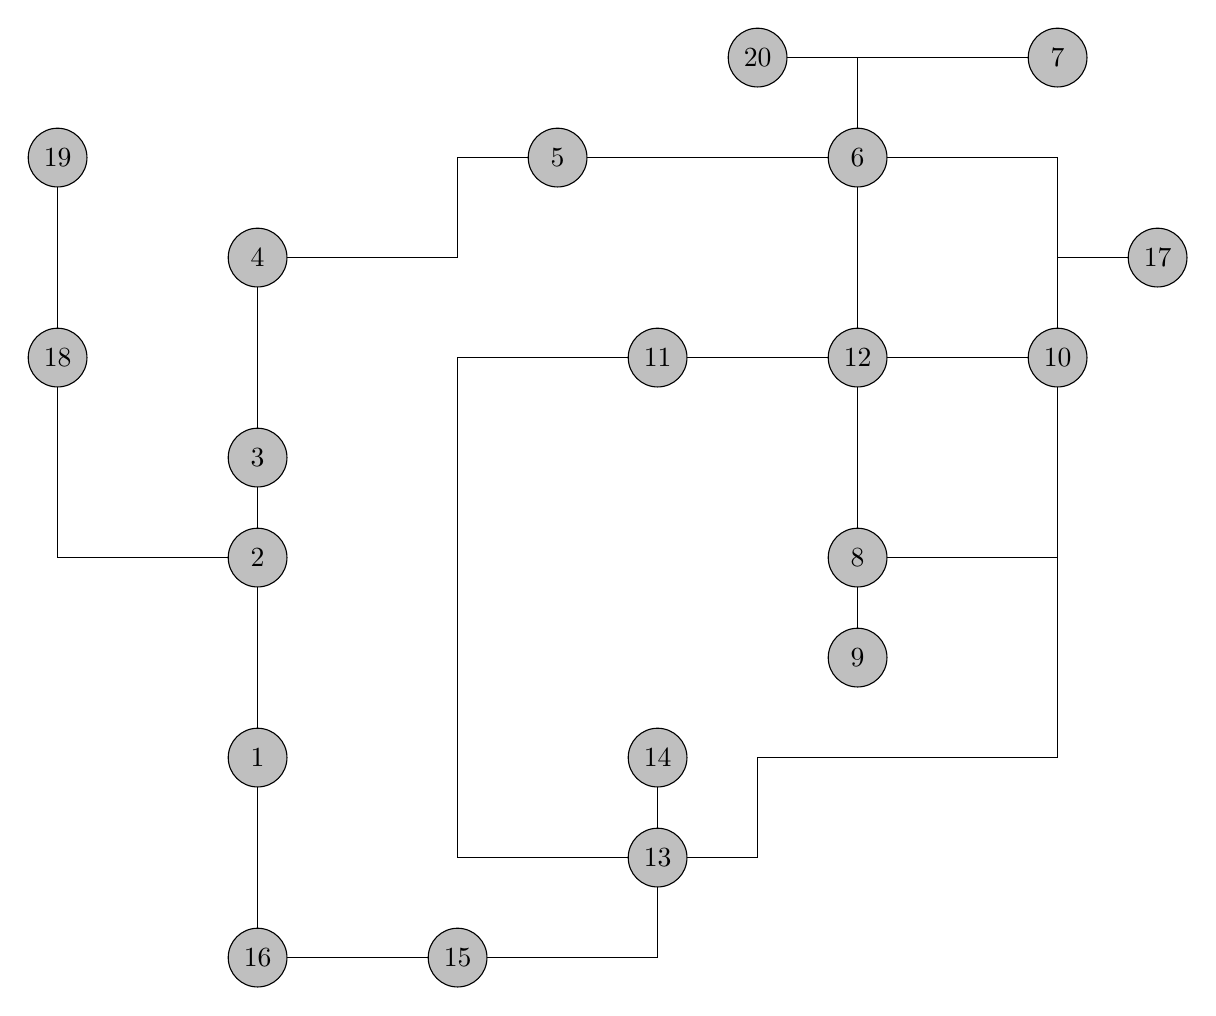
\begin{tikzpicture}[x=0.5in,y=0.5in,every node/.style={circle,fill=lightgray,draw=black,text width=1em,align=center}]
    \draw (2,0) -- (2,7) -- (4,7) -- (4,8) -- (10,8) --
          (10,2) -- (7,2) -- (7,1) -- (6,1) -- (6,0) -- (2,0);
    \draw (8,9) -- (8,3);
    \draw (8,4) -- (10,4);
    \draw (7,9) -- (10,9);
    \draw (10,6) -- (4,6) -- (4,1) -- (6,1);
    \draw (10,7) -- (11,7);
    \draw (2,4) -- (0,4) -- (0,8);
    \draw (6,1) -- (6,2);

    \node at (2,2) {1};
    \node at (2,4) {2};
    \node at (2,5) {3};
    \node at (2,7) {4};
    \node at (5,8) {5};
    \node at (8,8) {6};
    \node at (10,9) {7};
    \node at (8,4) {8};
    \node at (8,3) {9};
    \node at (10,6) {10};
    \node at (6,6) {11};
    \node at (8,6) {12};
    \node at (6,1) {13};
    \node at (6,2) {14};
    \node at (4,0) {15};
    \node at (2,0) {16};
    \node at (11,7) {17};
    \node at (0,6) {18};
    \node at (0,8) {19};
    \node at (7,9) {20};
  \end{tikzpicture}
\end{center}

% Include below for aucTeX integration
%%% Local Variables:
%%% mode: latex
%%% TeX-master: "../mapp-challenge-18-game-book"
%%% End:
